\subchapter{Application optimization}{Optimize the size and startup time
of your application}

\section{Measuring}

We have already measured application startup time in the previous lab.

\section{Remove unnecessary functionality}

\subsection{Compiling ffmpeg with a reduced configuration}

In our system, we use a generic version of \code{ffmpeg} that was built
with support for too many codecs and options that we actually do not
need in our very special case.

So, let's try to find out what the minimum requirements for
\code{ffmpeg} are.

A first thing to do is to look at the {\code ffmpeg} logs:

{\scriptsize
\begin{verbatim}
Input #0, video4linux2,v4l2, from '/dev/video0':
  Duration: N/A, start: 93.369296, bitrate: N/A
    Stream #0:0: Video: mjpeg (Baseline), yuvj422p(pc, bt470bg/unknown/unknown), 544x288, 30 fps, 30 tbr, 1000k tbn, 1000k tbc
Stream mapping:
  Stream #0:0 -> #0:0 (mjpeg (native) -> rawvideo (native))
Press [q] to stounable to decode APP fields: Invalid data found when processing input
[swscaler @ 0x80f50] deprecated pixel format used, make sure you did set range correctly
[swscaler @ 0x80f50] No accelerated colorspace conversion found from yuv422p to rgb565le.
Output #0, fbdev, to '/dev/fb0':
  Metadata:
    encoder         : Lavf58.29.100
    Stream #0:0: Video: rawvideo (RGB[16] / 0x10424752), rgb565le, 544x288, q=2-31, 75202 kb/s, 30 fps, 30 tbn, 30 tbc
    Metadata:
      encoder         : Lavc58.54.100 rawvideo
\end{verbatim}
}

Here we see that \code{ffmpeg} is using:
\begin{itemize}
\item Input from a \code{video4linux} device, decoding an \code{mjpeg}
stream.
\item Encoding a \code{rawvideo} stream, written to an
\code{fbdev} output device.
\item A software scaler to resize the input video for our LCD screen
\end{itemize}

Let's check \code{ffmpeg}'s \code{configure} script, and see what its
options are:

\begin{verbatim}
cd ~/boot-time-labs/rootfs/buildroot/output/build/ffmpeg-4.4.4
./configure --help
\end{verbatim}

We see that \code{configure} has precisely three interesting options:
\code{--list-encoders}, \code{--list-decoders}, \code{--list-filters},
\code{--list-outdevs} and \code{--list-indevs}.

Run \code{configure} with each of those and recognize the features that
we need to enable.

Following these findings, here's how we are going to modify Buildroot's
configuration for \code{ffmpeg}.

\begin{verbatim}
cd ~/boot-time-labs/rootfs/buildroot/
make menuconfig
\end{verbatim}

In Buildroot's configuration interface, in \code{ffmpeg} options:

\begin{itemize}
\item Set \code{Enabled encoders} to \code{rawvideo}
\item Set \code{Enabled decoders} to \code{mjpeg}
\item Empty the \code{Enabled muxers}, \code{Enabled demuxers},
      \code{Enabled parsers}, \code{Enabled bitstreams} and \code{Enabled protocols} settings.
\item Set \code{Enabled filters} to \code{scale}
\item For \code{Enable output devices} and \code{Enable input devices},
      individual device selection is not possible, so we will configure
      devices manually in the next field. So, empty such settings.
\item Set \code{Additional parameters for ./configure} to\\
      \code{--enable-indev=v4l2 --enable-outdev=fbdev}
\end{itemize}

Now, let's get Buildroot to recompile \code{ffmpeg}, taking our new
settings into account:

\begin{verbatim}
make ffmpeg-dirclean
make
\end{verbatim}

You can now fill the \code{~/boot-time-labs/results/application-size.ods} spreadsheet,
reusing data from the previous lab:

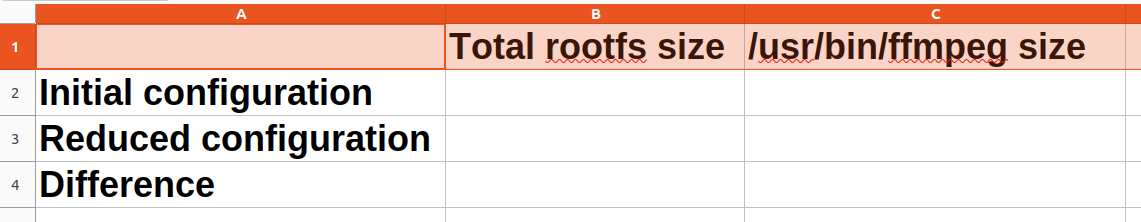
\includegraphics[width=0.7\textwidth]{labs/boot-time-application/application-size.png}

Do you expect to see differences in execution time, with a reduced
configuration? Run the measures with \code{time} again, and compare with
what you got during the previous lab.

If the results surprise you, don't hesitate to show them to your
instructor ask for her/his opinion.

\subsection{Trying to remove further features}

Looking at the \code{ffmpeg} log which displays enabled configuration
settings, try to find further configuration switches which can be
removed without breaking the player in our particular system.

\subsection{Further analysis of the application}

With a build system like Buildroot, it's easy to add performance
analysis and debugging utilities.

Configure Buildroot to add \code{strace} to your root
filesystem. You will find the corresponding configuration option in
\code{Package selection for the target} and then in \code{Debugging,
profiling and benchmark}.

Run Buildroot and reflash your device as usual.

\subsection{Tracing and profiling with strace}

With \code{strace}'s help, you can already have a pretty good understanding
of how your application spends its time. You can see all the system
calls that it makes and knowing the application, you can guess in which
part of the code it is at a given time.

You can also spot unnecessary attempts to open files that do not exist,
multiple accesses to the same file, or more generally things that the
program was not supposed to do. All these correspond to opportunities
to fix and optimize your application.

Once the board has booted, run \code{strace} on the video player
application:

\begin{verbatim}
strace -tt -f -o /tmp/strace.log ffmpeg -f video4linux2 -video_size 544x288 \
-input_format mjpeg -i /dev/video0 -pix_fmt rgb565le -f fbdev /dev/fb0
\end{verbatim}

Also have \code{strace} generate a summary:

\begin{verbatim}
strace -c -f -o /tmp/strace-summary.log ffmpeg ...
\end{verbatim}

Take some time to read \code{/tmp/strace.log}\footnote{
At this stage, when you have to open files directly on the
board, some familiarity with the basic commands of the \code{vi} editor
becomes useful. See
\url{https://bootlin.com/doc/command_memento.pdf} for a basic
command summary. Otherwise, you can use the more rudimentary \code{more}
command. You can also copy the files to your PC, using a USB drive, for
example.}, and see everything that the program is doing. Don't hesitate
to lookup the ioctl codes on the Internet to have an idea about what's
going on between the player, the camera and the display.

Also have a look at \code{/tmp/strace-summary.log}. You will find the number
of errors trying to open files that do not exist, and where most time is
spent, for example. You can also count the number of memory allocations
(using the \code{mmap2} system call).

\section{Optimizing necessary functionality}

At this stage, there is nothing more we can really do to further
optimize \code{ffmpeg}, unless we are ready to dig into the code and
make changes.

However, if the player was your own application, I'm sure this would
help to understand how it's actually behaving and how to improve it to
make it even faster and smaller.

\section{Putting things back together}

Now that we have analyzed the execution of the video player, let's
restore the normal configuration for the system:

\begin{itemize}
\item Remove support for \code{strace}
\item Restore the
      \code{0001-ffmpeg-log-notification-after-first-frame.patch} patch,
      replacing the most recently applied patch.
\item Restoring the automatic execution of \code{ffmpeg} in
      \code{/etc/init.d/S50playvideo}.
\end{itemize}


As explained in the Buildroot
manual\footnote{https://buildroot.org/downloads/manual/manual.html\#full-rebuild},
you need to make a full rebuild after disabling packages (such as
\code{strace} in our case). Otherwise, such packages will still be present in the
filesystem image. Fortunately, full rebuilds are now fast with Buildroot
when it's using a prebuilt toolchain:

\begin{verbatim}
make clean
make
\end{verbatim}

Update your root filesystem and then reboot your system through \code{grabserial},
copying the output to \code{~/logs/application.log}.

Run the experiment 3 times and fill the \code{~/boot-time-labs/results/application-optimizations.ods}
spreadsheet:

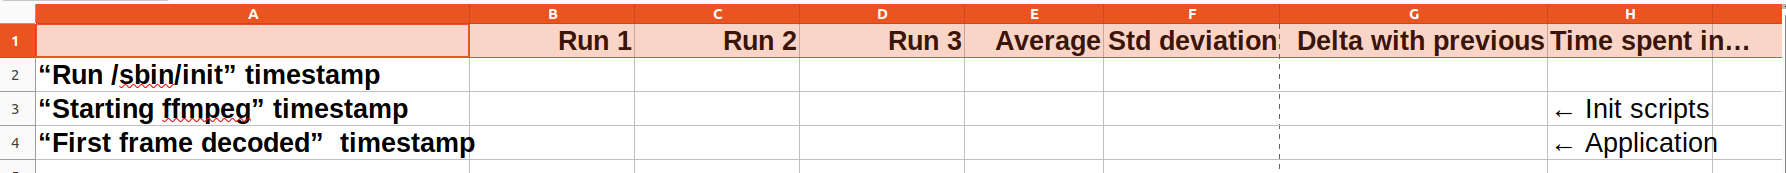
\includegraphics[width=\textwidth]{labs/boot-time-application/application-optimizations.png}

